

\documentclass[tikz]{standalone}

\usepackage[english]{babel}
\usepackage[utf8]{inputenc}
\usepackage{amsfonts,amssymb,amsbsy}
\usepackage{xcolor}

\usepackage{tikz}
\usetikzlibrary{arrows.meta, positioning, quotes, calc, intersections, decorations.pathreplacing}

\begin{document}

	\begin{tikzpicture}
	
		\tikzset{
			myline/.style={draw=black!50!white, line width=0.4mm, rounded corners},
			myarrow/.style={myline, -{Latex[width=0.2cm, length=0.3cm]}},
			fontstyle/.style={font=\footnotesize},
			labelstyle/.style={fontstyle, yshift=-12mm}
		}
	
		% Set images and labels
		\path node[outer sep=-4mm] (0,0) (mol) {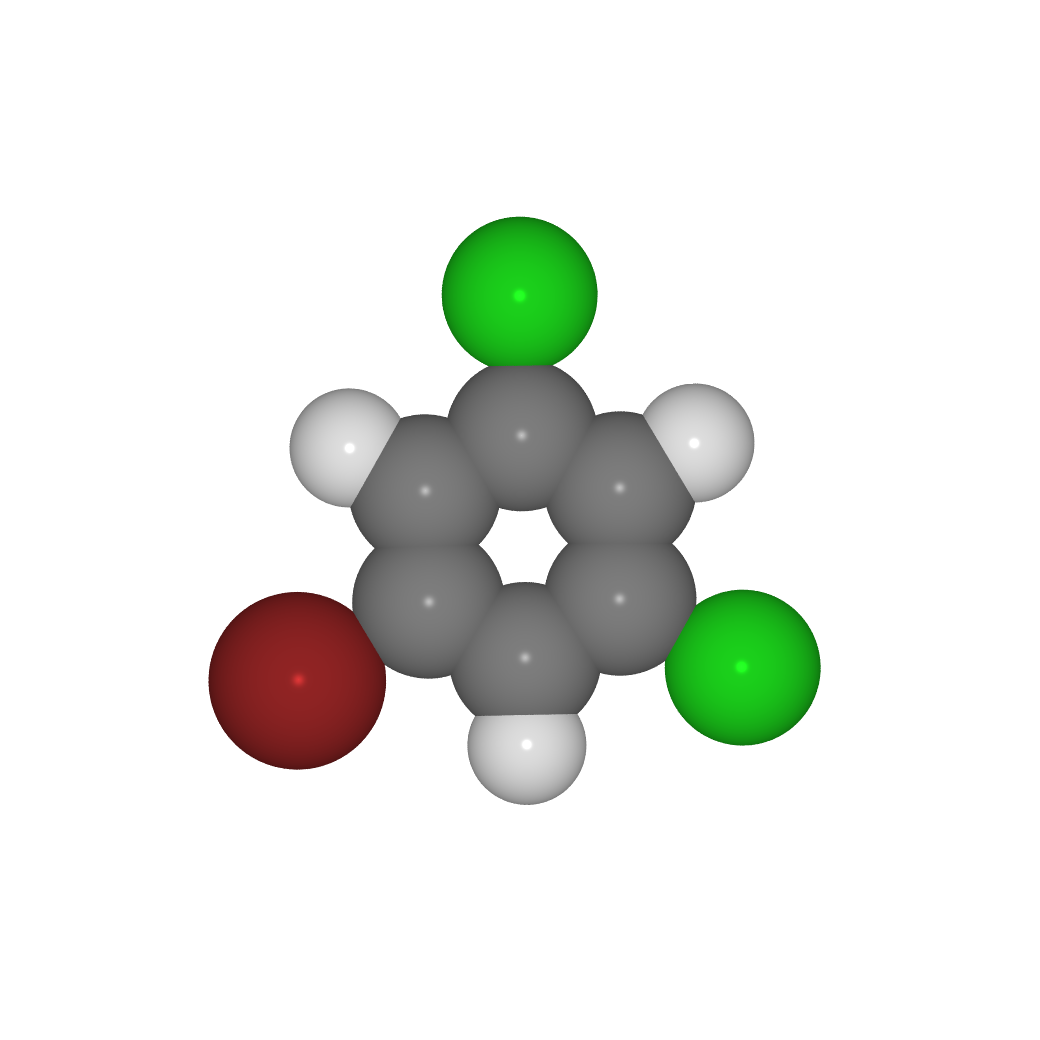
\includegraphics[width=20mm]{../data/BCB/mol.png}} node[labelstyle, align=center, yshift=2mm] {Molecule\\geometry}
		++(30mm,13mm) node (es) {\includegraphics[width=20mm]{./images/es.png}} node[labelstyle] {ES field}
		++(0,-26mm) node (vdw) {\includegraphics[width=20mm]{./images/vdw.png}} node[labelstyle] {vdW Spheres}
		
		++(35mm, 0) node (mask) {\includegraphics[width=20mm]{./images/vdw_mask.png}} node[labelstyle] {Mask}
		++(0, 26mm) node[draw, circle, myline, minimum size=5mm, inner sep=0, outer sep=2mm] (times) {}
		node[text=black!50!white, xshift=0.05mm, yshift=-0.05mm] {$\boldsymbol{\times}$}
		
		++(35mm, 0)  node (esmap) {\includegraphics[width=20mm]{./images/es_cut.png}} node[labelstyle] {ES Map};
		
		% Draw arrows
		\draw[myarrow] (mol) -- (es);
		\draw[myarrow] (mol) -- (vdw);
		\draw[myarrow] (vdw) -- (mask);
		\draw[myarrow] (mask) -- (times);
		\draw[myarrow] (es) -- (times);
		\draw[myarrow] (times) -- (esmap);
		
	
ra	\end{tikzpicture}
	
	
\end{document}